\documentclass[aspectratio=169]{beamer}
\usetheme{simple}

\RequirePackage[l2tabu, orthodox]{nag}


% \usepackage[left=1.in, right=1.in, top=1.25in, bottom=1.25in]{geometry}

% FONTS
%\usepackage[T1]{fontenc}

% Replace default Latin Modern typewriter with its proportional counterpart
% http://www.tug.dk/FontCatalogue/lmoderntypewriterprop/
%\renewcommand*\ttdefault{lmvtt}


%%% OPTION 1 - Fourier Math + New Century Schoolbook + ParaType Sans

% % Import Fourier Math (this imposes its own New Century Schoolbook type)
% % http://www.ctan.org/tex-archive/fonts/fouriernc/
%\usepackage{fouriernc}
%\usepackage{amsmath}
% % Replace with TeX Gyre Schola version of New Century Schoolbook (must scale!)
% % http://www.tug.dk/FontCatalogue/tgschola/
%\usepackage[scale=0.92]{tgschola}
%\usepackage[scaled=0.88]{PTSans}

%% OPTION 2 - MathDesign Math + Bitstream Charter + ParaType Sans

% Import MathDesign (this brings along Bitstream Charter)
% http://www.ctan.org/tex-archive/fonts/mathdesign/
\usepackage[bitstream-charter]{mathdesign}
\usepackage{amsmath}
\usepackage[scaled=0.92]{PTSans}


% %%% OPTION 3 - MTPRO 2 Math + Termes Times + ParaType Sans

% \usepackage{tgtermes}
% \usepackage{amsmath}
% \usepackage[subscriptcorrection,
%             amssymbols,
%             mtpbb,
%             mtpcal,
%             nofontinfo  % suppresses all warnings
%            ]{mtpro2}
% \usepackage{scalefnt,letltxmacro}
% \LetLtxMacro{\oldtextsc}{\textsc}
% \renewcommand{\textsc}[1]{\oldtextsc{\scalefont{1.10}#1}}
% \usepackage[scaled=0.92]{PTSans}

% Use default fonts here
\usepackage{amsmath}
\usepackage{amssymb}

% \usepackage{titling}

% % COLOR
% \usepackage[table,usenames,dvipsnames]{xcolor}
\definecolor{shadecolor}{gray}{0.9}

% SPACING and TEXT
\usepackage[final,expansion=alltext]{microtype}
\usepackage[english]{babel}
\usepackage[parfill]{parskip}
\usepackage{afterpage}
\usepackage{framed}
\usepackage{verbatim}
\usepackage{setspace}

\newenvironment{exercise}[1]
{
    \itshape
    \paragraph{Exercise: \textit{#1}}
}
{ 
}


% \usepackage[bottom]{footmisc}
\usepackage[symbol]{footmisc}
\renewcommand{\thefootnote}{\arabic{footnote}}


% FIGURES
\usepackage{graphicx}
\usepackage[labelfont={it, small}, 
            textfont={small,singlespacing},
            % justification={justified,RaggedRight},
            singlelinecheck=false,
            margin=0pt]{caption}
\usepackage[format=hang]{subcaption}
% \usepackage{ccaption}

% % APPENDIX FIGURES
% \usepackage{chngcntr}

% % TABLES
% \usepackage{booktabs}
% \usepackage{longtable}
% \usepackage{hhline}

% ALGORITHMS
\usepackage[algoruled]{algorithm2e}
\usepackage{listings}
\usepackage{fancyvrb}
\fvset{fontsize=\normalsize}

% % THEOREMS
\usepackage{amsthm}
\newtheorem{proposition}{Proposition}
% \newtheorem{lemma}{Lemma}

% % BIBLIOGRAPHY
\usepackage{natbib}

% HYPERREF
% \usepackage[colorlinks,linktoc=all]{hyperref}
% \usepackage[all]{hypcap}
% \hypersetup{citecolor=MidnightBlue}
% \hypersetup{linkcolor=black}
% \hypersetup{urlcolor=MidnightBlue}

% % CLEVEREF must come after HYPERREF
% \usepackage[nameinlink]{cleveref}

% % ACRONYMS
% \usepackage[acronym,smallcaps,nowarn]{glossaries}
% % \makeglossaries

% % COLOR DEFINITIONS
\newcommand{\red}[1]{\textcolor{BrickRed}{#1}}
\newcommand{\orange}[1]{\textcolor{BurntOrange}{#1}}
\newcommand{\green}[1]{\textcolor{OliveGreen}{#1}}
\newcommand{\blue}[1]{\textcolor{MidnightBlue}{#1}}
\newcommand{\gray}[1]{\textcolor{black!60}{#1}}

% LISTINGS DEFINTIONS
\lstdefinestyle{mystyle}{
    commentstyle=\color{OliveGreen},
    keywordstyle=\color{BurntOrange},
    numberstyle=\tiny\color{black!60},
    stringstyle=\color{MidnightBlue},
    basicstyle=\ttfamily,
    breakatwhitespace=false,
    breaklines=true,
    captionpos=b,
    keepspaces=true,
    numbers=left,
    numbersep=5pt,
    showspaces=false,
    showstringspaces=false,
    showtabs=false,
    tabsize=2
}
\lstset{style=mystyle}

\usepackage[colorinlistoftodos,
            prependcaption,
            textsize=small,
            backgroundcolor=yellow,
            linecolor=lightgray,
            bordercolor=lightgray]{todonotes}

\usepackage{soul}

\usepackage{media9}
% !TEX root = template.tex

% \DeclareRobustCommand{\mb}[1]{\ensuremath{\boldsymbol{\mathbf{#1}}}}
\DeclareRobustCommand{\mb}[1]{\boldsymbol{#1}}

% \newcommand{\KL}[2]{\ensuremath{\textrm{KL}\PARENS{#1\;\|\;#2}}}
\DeclareRobustCommand{\KL}[2]{\ensuremath{\textrm{KL}\left(#1\;\|\;#2\right)}}

\DeclareMathOperator*{\argmax}{arg\,max}
\DeclareMathOperator*{\argmin}{arg\,min}

\renewcommand{\mid}{~\vert~}
\newcommand{\given}{\,|\,}
\newcommand{\iid}[1]{\stackrel{\text{iid}}{#1}}

\newcommand{\mba}{\mb{a}}
\newcommand{\mbb}{\mb{b}}
\newcommand{\mbc}{\mb{c}}
\newcommand{\mbd}{\mb{d}}
\newcommand{\mbe}{\mb{e}}
% \newcommand{\mbf}{\mb{f}}
\newcommand{\mbg}{\mb{g}}
\newcommand{\mbh}{\mb{h}}
\newcommand{\mbi}{\mb{i}}
\newcommand{\mbj}{\mb{j}}
\newcommand{\mbk}{\mb{k}}
\newcommand{\mbl}{\mb{l}}
\newcommand{\mbm}{\mb{m}}
\newcommand{\mbn}{\mb{n}}
\newcommand{\mbo}{\mb{o}}
\newcommand{\mbp}{\mb{p}}
\newcommand{\mbq}{\mb{q}}
\newcommand{\mbr}{\mb{r}}
\newcommand{\mbs}{\mb{s}}
\newcommand{\mbt}{\mb{t}}
\newcommand{\mbu}{\mb{u}}
\newcommand{\mbv}{\mb{v}}
\newcommand{\mbw}{\mb{w}}
\newcommand{\mbx}{\mb{x}}
\newcommand{\mby}{\mb{y}}
\newcommand{\mbz}{\mb{z}}

\newcommand{\mbA}{\mb{A}}
\newcommand{\mbB}{\mb{B}}
\newcommand{\mbC}{\mb{C}}
\newcommand{\mbD}{\mb{D}}
\newcommand{\mbE}{\mb{E}}
\newcommand{\mbF}{\mb{F}}
\newcommand{\mbG}{\mb{G}}
\newcommand{\mbH}{\mb{H}}
\newcommand{\mbI}{\mb{I}}
\newcommand{\mbJ}{\mb{J}}
\newcommand{\mbK}{\mb{K}}
\newcommand{\mbL}{\mb{L}}
\newcommand{\mbM}{\mb{M}}
\newcommand{\mbN}{\mb{N}}
\newcommand{\mbO}{\mb{O}}
\newcommand{\mbP}{\mb{P}}
\newcommand{\mbQ}{\mb{Q}}
\newcommand{\mbR}{\mb{R}}
\newcommand{\mbS}{\mb{S}}
\newcommand{\mbT}{\mb{T}}
\newcommand{\mbU}{\mb{U}}
\newcommand{\mbV}{\mb{V}}
\newcommand{\mbW}{\mb{W}}
\newcommand{\mbX}{\mb{X}}
\newcommand{\mbY}{\mb{Y}}
\newcommand{\mbZ}{\mb{Z}}

\newcommand{\mbalpha}{\mb{\alpha}}
\newcommand{\mbbeta}{\mb{\beta}}
\newcommand{\mbdelta}{\mb{\delta}}
\newcommand{\mbepsilon}{\mb{\epsilon}}
\newcommand{\mbchi}{\mb{\chi}}
\newcommand{\mbeta}{\mb{\eta}}
\newcommand{\mbgamma}{\mb{\gamma}}
\newcommand{\mbiota}{\mb{\iota}}
\newcommand{\mbkappa}{\mb{\kappa}}
\newcommand{\mblambda}{\mb{\lambda}}
\newcommand{\mbmu}{\mb{\mu}}
\newcommand{\mbnu}{\mb{\nu}}
\newcommand{\mbomega}{\mb{\omega}}
\newcommand{\mbphi}{\mb{\phi}}
\newcommand{\mbpi}{\mb{\pi}}
\newcommand{\mbpsi}{\mb{\psi}}
\newcommand{\mbrho}{\mb{\rho}}
\newcommand{\mbsigma}{\mb{\sigma}}
\newcommand{\mbtau}{\mb{\tau}}
\newcommand{\mbtheta}{\mb{\theta}}
\newcommand{\mbupsilon}{\mb{\upsilon}}
\newcommand{\mbvarepsilon}{\mb{\varepsilon}}
\newcommand{\mbvarphi}{\mb{\varphi}}
\newcommand{\mbvartheta}{\mb{\vartheta}}
\newcommand{\mbvarrho}{\mb{\varrho}}
\newcommand{\mbxi}{\mb{\xi}}
\newcommand{\mbzeta}{\mb{\zeta}}

\newcommand{\mbDelta}{\mb{\Delta}}
\newcommand{\mbGamma}{\mb{\Gamma}}
\newcommand{\mbLambda}{\mb{\Lambda}}
\newcommand{\mbOmega}{\mb{\Omega}}
\newcommand{\mbPhi}{\mb{\Phi}}
\newcommand{\mbPi}{\mb{\Pi}}
\newcommand{\mbPsi}{\mb{\Psi}}
\newcommand{\mbSigma}{\mb{\Sigma}}
\newcommand{\mbTheta}{\mb{\Theta}}
\newcommand{\mbUpsilon}{\mb{\Upsilon}}
\newcommand{\mbXi}{\mb{\Xi}}

\newcommand{\dif}{\mathop{}\!\mathrm{d}}
\newcommand{\diag}{\textrm{diag}}
\newcommand{\supp}{\textrm{supp}}
\newcommand{\Tr}{\textrm{Tr}}

\newcommand{\E}{\mathbb{E}}
\newcommand{\Var}{\mathbb{V}\textrm{ar}}
% \newcommand{\given}{\mid}

\newcommand{\bbA}{\mathbb{A}}
\newcommand{\bbB}{\mathbb{B}}
\newcommand{\bbC}{\mathbb{C}}
\newcommand{\bbD}{\mathbb{D}}
\newcommand{\bbE}{\mathbb{E}}
\newcommand{\bbF}{\mathbb{F}}
\newcommand{\bbG}{\mathbb{G}}
\newcommand{\bbH}{\mathbb{H}}
\newcommand{\bbI}{\mathbb{I}}
\newcommand{\bbJ}{\mathbb{J}}
\newcommand{\bbK}{\mathbb{K}}
\newcommand{\bbL}{\mathbb{L}}
\newcommand{\bbM}{\mathbb{M}}
\newcommand{\bbN}{\mathbb{N}}
\newcommand{\bbO}{\mathbb{O}}
\newcommand{\bbP}{\mathbb{P}}
\newcommand{\bbQ}{\mathbb{Q}}
\newcommand{\bbR}{\mathbb{R}}
\newcommand{\bbS}{\mathbb{S}}
\newcommand{\bbT}{\mathbb{T}}
\newcommand{\bbU}{\mathbb{U}}
\newcommand{\bbV}{\mathbb{V}}
\newcommand{\bbW}{\mathbb{W}}
\newcommand{\bbX}{\mathbb{X}}
\newcommand{\bbY}{\mathbb{Y}}
\newcommand{\bbZ}{\mathbb{Z}}

\newcommand{\cA}{\mathcal{A}}
\newcommand{\cB}{\mathcal{B}}
\newcommand{\cC}{\mathcal{C}}
\newcommand{\cD}{\mathcal{D}}
\newcommand{\cE}{\mathcal{E}}
\newcommand{\cF}{\mathcal{F}}
\newcommand{\cG}{\mathcal{G}}
\newcommand{\cH}{\mathcal{H}}
\newcommand{\cI}{\mathcal{I}}
\newcommand{\cJ}{\mathcal{J}}
\newcommand{\cK}{\mathcal{K}}
\newcommand{\cL}{\mathcal{L}}
\newcommand{\cM}{\mathcal{M}}
\newcommand{\cN}{\mathcal{N}}
\newcommand{\cO}{\mathcal{O}}
\newcommand{\cP}{\mathcal{P}}
\newcommand{\cQ}{\mathcal{Q}}
\newcommand{\cR}{\mathcal{R}}
\newcommand{\cS}{\mathcal{S}}
\newcommand{\cT}{\mathcal{T}}
\newcommand{\cU}{\mathcal{U}}
\newcommand{\cV}{\mathcal{V}}
\newcommand{\cW}{\mathcal{W}}
\newcommand{\cX}{\mathcal{X}}
\newcommand{\cY}{\mathcal{Y}}
\newcommand{\cZ}{\mathcal{Z}}

\newcommand{\trans}{\mathsf{T}}
\newcommand{\naturals}{\mathbb{N}}
\newcommand{\reals}{\mathbb{R}}
\newcommand{\const}{\mathrm{const}}

\newcommand{\distBernoulli}{\mathrm{Bern}}
\newcommand{\distBeta}{\mathrm{Beta}}
\newcommand{\distBinomial}{\mathrm{Bin}}
\newcommand{\distCategorical}{\mathrm{Cat}}
\newcommand{\distDirichlet}{\mathrm{Dir}}
\newcommand{\distExp}{\mathrm{Exp}}
\newcommand{\distGamma}{\mathrm{Gamma}}
\newcommand{\distMNIW}{\mathrm{MNIW}}
\newcommand{\distMultinomial}{\mathrm{Mult}}
\newcommand{\distNegBinomial}{\mathrm{NB}}
\newcommand{\distNormal}{\mathcal{N}}
\newcommand{\distPoisson}{\mathrm{Po}}
\newcommand{\distPoissonProcess}{\mathrm{PP}}
\newcommand{\distPolyaGamma}{\mathrm{PG}}
\newcommand{\distUniform}{\mathrm{Unif}}
\newcommand{\distInvChiSq}{\mathrm{Inv-}\chi^2}

\newcommand{\dtmax}{\Delta t_{\mathsf{max}}}

\newcommand{\mbzero}{\boldsymbol{0}}
% \newacronym{KL}{kl}{Kullback-Leibler}
\newacronym{ELBO}{elbo}{\emph{evidence lower bound}}
\newacronym{EM}{em}{\emph{expectation-maximization}}
\newacronym{PPCA}{ppca}{probabilistic principal components analysis}

\newacronym{SVI}{svi}{stochastic variational inference}
\newacronym{GMM}{gmm}{Gaussian mixture model}
\newacronym{HMM}{hmm}{hidden Markov model}
\newacronym{IO-HMM}{io-hmm}{input-output hidden Markov model}
\newacronym{LDS}{lds}{linear dynamical system}
\newacronym{SLDS}{slds}{switching linear dynamical system}
\newacronym{AR-HMM}{ar-hmm}{autoregressive hidden Markov model}


\title{STATS271/371: Applied Bayesian Statistics}
\subtitle{Bayesian Mixture Models and (Collapsed) Gibbs Sampling}
\author{Scott Linderman}
\date{\today}


\begin{document}


\maketitle

\begin{frame}{Box's Loop}
\begin{center}
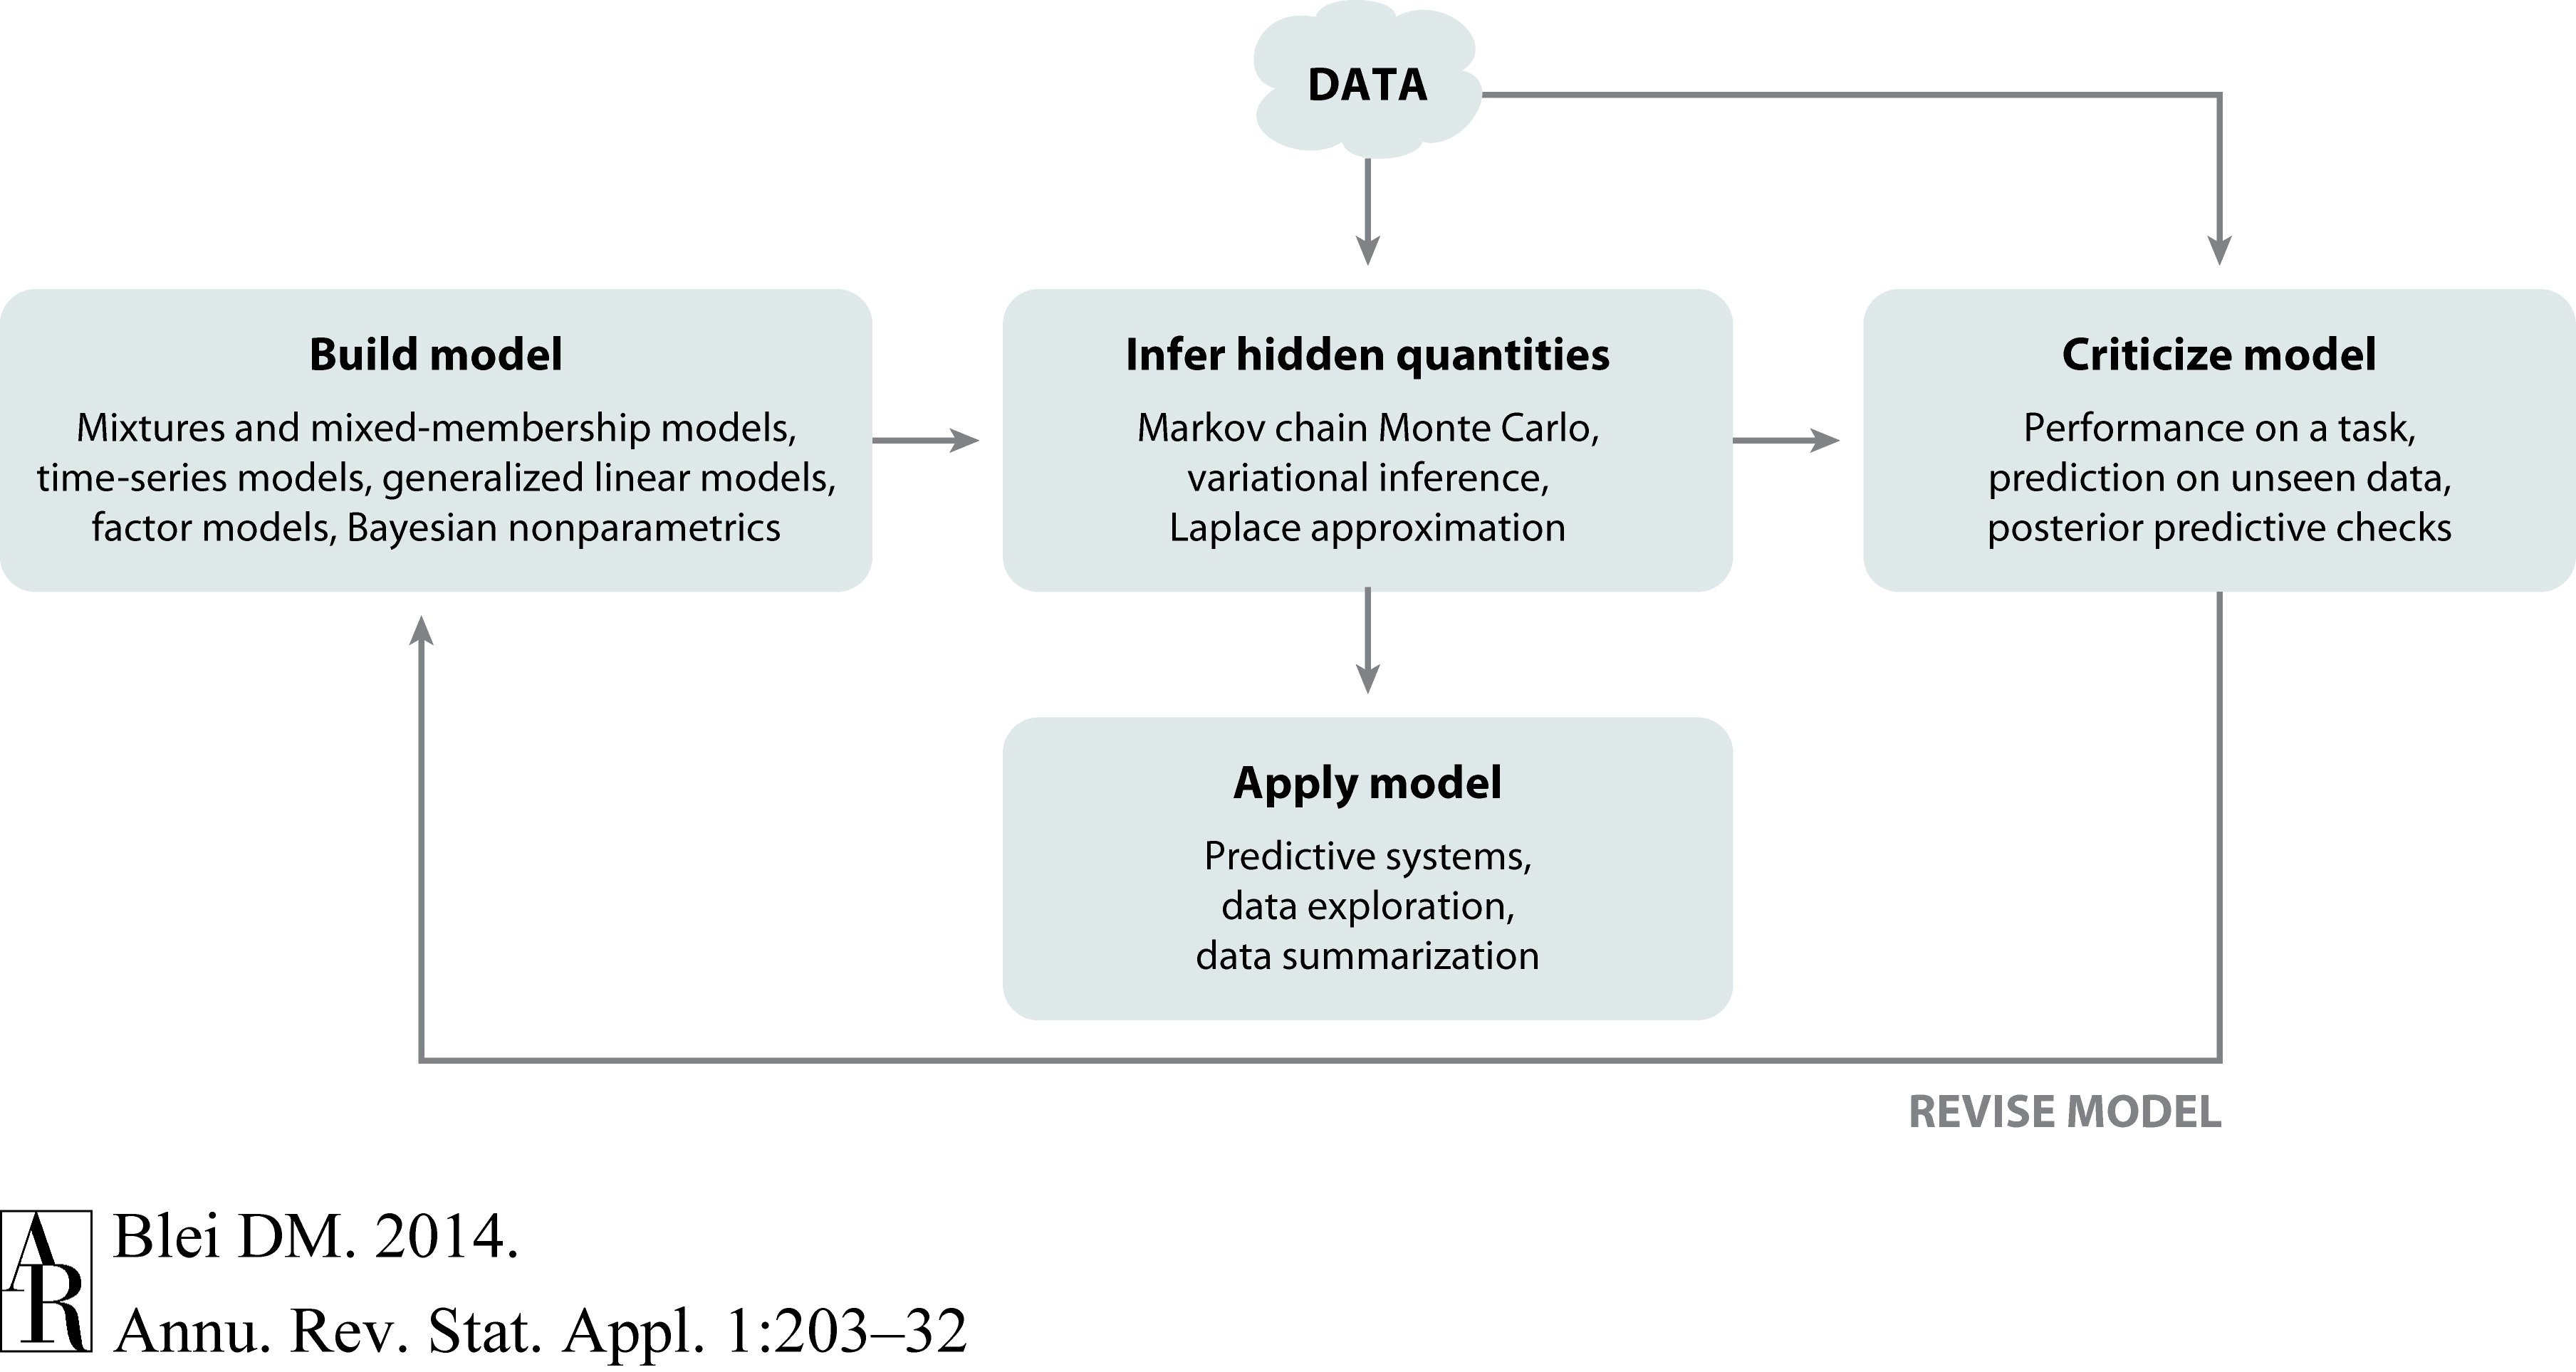
\includegraphics[width=.85\linewidth]{figures/lap1/boxsloop.jpeg}\\
\end{center} 
\begin{flushright}
{\footnotesize Blei, \textit{Ann. Rev. Stat. App.} 2014.}
\end{flushright}
\end{frame}

\begin{frame}{Lap 4: Bayesian Mixture Models and (Collapsed) Gibbs Sampling}
\begin{itemize}
    \item \hyperref[sec:mixtures]{\textbf{Model:} Bayesian mixture models}
    \item \hyperref[sec:gibbs]{\textbf{Algorithm:} Gibbs sampling}
    \item \hyperref[sec:ppcs]{\textbf{Criticism:} Posterior predictive checks}
    \item \hyperref[sec:collapsed_gibbs]{\textbf{Algorithm II:} Collapsed Gibbs sampling}
\end{itemize}
\end{frame}


\section{Model: Bayesian Mixture Models}
\label{sec:mixtures}

\begin{frame}{Motivation: Clustering scRNA-seq data}
\centering
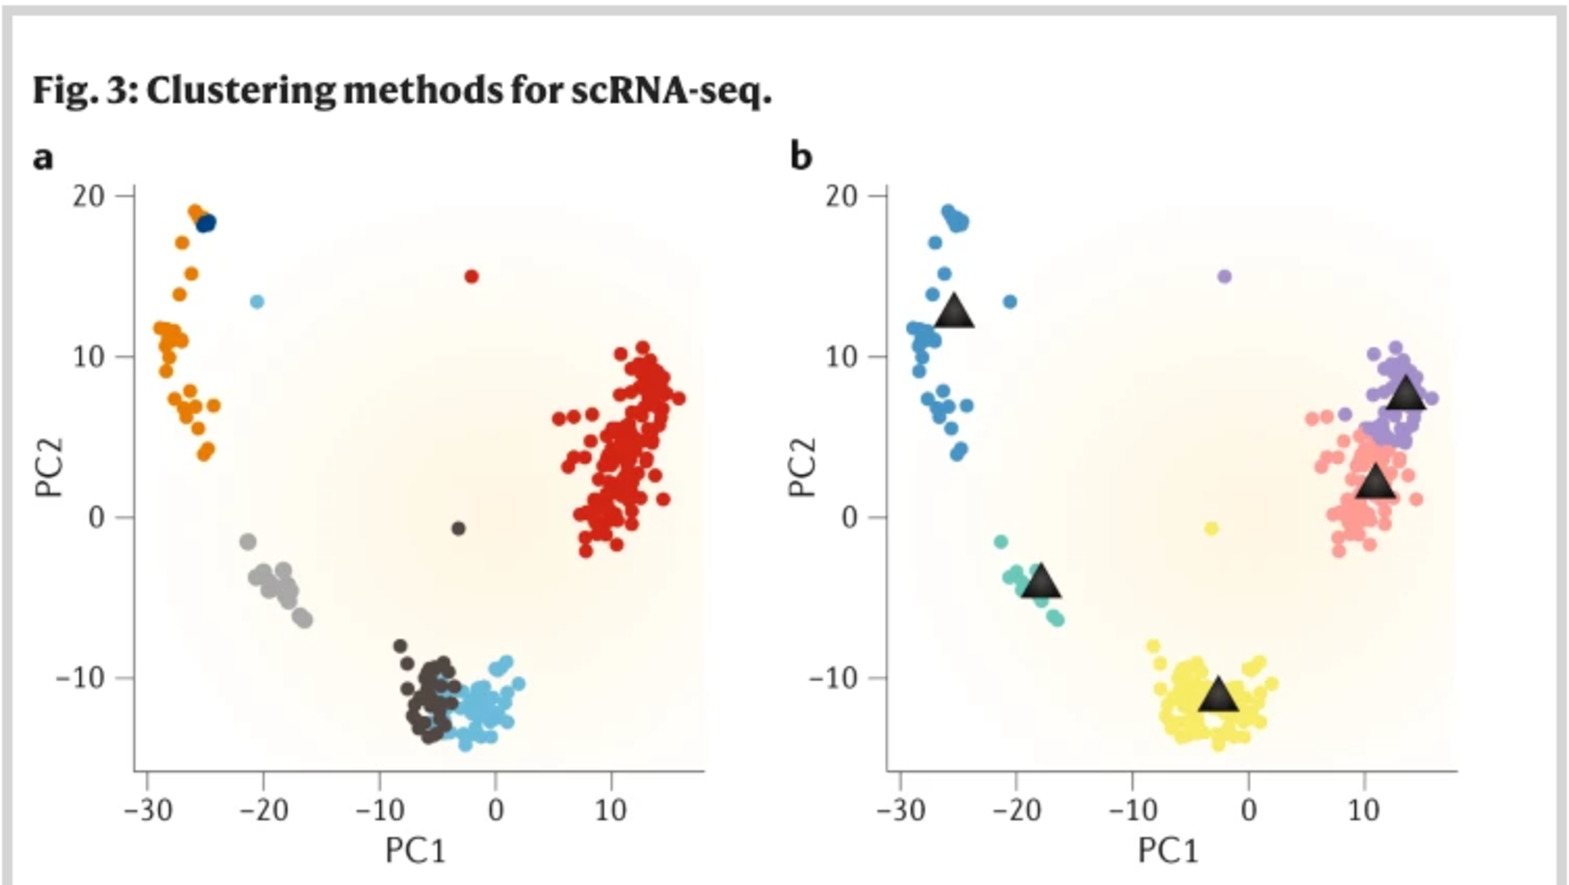
\includegraphics[width=0.7\textwidth]{figures/lap4/scrnaseq.pdf}

From \citet{Kiselev2019-bt}
\end{frame}

\begin{frame}{Motivation: Foreground/background segmentation}
\centering
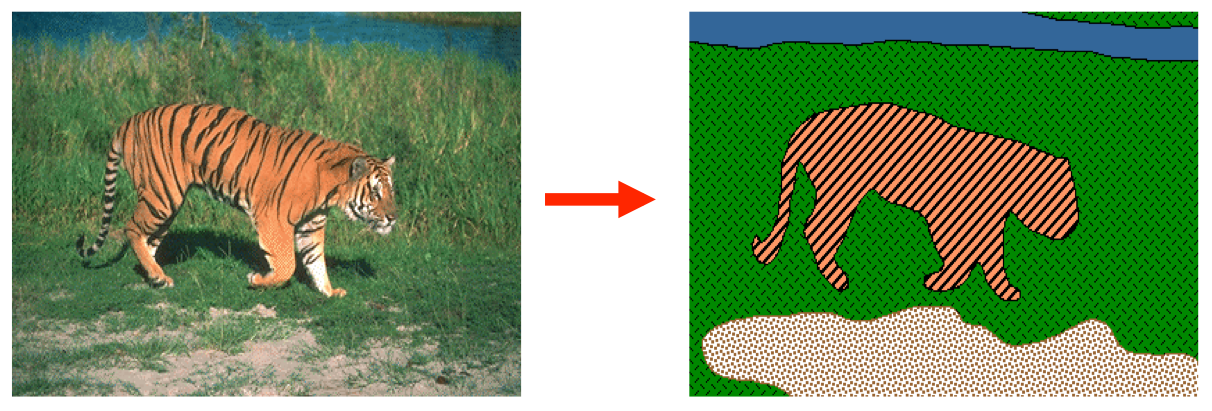
\includegraphics[width=0.9\textwidth]{figures/lap4/segmentation.png}

{\footnotesize \url{https://ai.stanford.edu/~syyeung/cvweb/tutorial3.html}}
\end{frame}

\begin{frame}{Motivation: Density estimation}
\centering
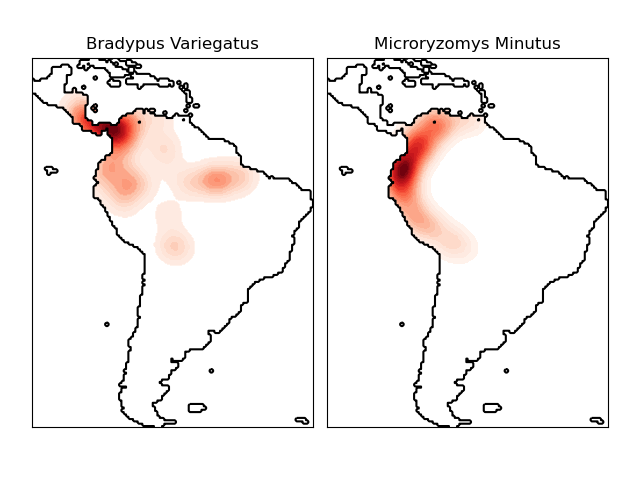
\includegraphics[width=0.65\textwidth]{figures/lap4/sphx_glr_plot_species_kde_001.png}
{\footnotesize \url{https://scikit-learn.org/stable/auto_examples/neighbors/plot_species_kde.html}}
\end{frame}

\begin{frame}{Notation}
    
\textbf{Constants: } Let
\begin{itemize}
    \item $N$ denote the number of data points.
    \item $K$ denote the number of mixture components (i.e. clusters)
\end{itemize}

\textbf{Data:} Let
\begin{itemize}
    \item $\mbx_n \in \reals^D$ denote the $n$-th data point.
\end{itemize}

\textbf{Latent Variables:} Let
\begin{itemize}
    \item $z_n \in \{1, \ldots, K\}$ denote the \textit{assignment} of the $n$-th data point.
\end{itemize}
\end{frame}

\begin{frame}{Notation II}

\textbf{Parameters:} Let
\begin{itemize}
    \item $\mbeta_k$ denote the \textit{natural parameters} of component $k$
    \item $\mbpi \in \Delta_K$ denote the component \textit{proportions} (i.e. probabilities).
\end{itemize}

\textbf{Hyperparameters:} Let
\begin{itemize}
    \item $\mbphi, \nu$ denote hyperparameters of the prior on $\mbeta$
    \item $\mbalpha \in \reals_+^{K}$ denote the concentration of the prior on proportions.
\end{itemize}
    
\end{frame}

\begin{frame}{Generative Model}

\begin{enumerate}
    \item Sample the proportions from a Dirichlet prior:
    \begin{align}
        \mbpi &\sim \distDirichlet(\mbalpha) \hspace{10em}
    \end{align}
    
    \item Sample the parameters for each component:
    \begin{align}
        \mbeta_k &\iid{\sim} p(\mbeta \mid \mbphi, \nu) \qquad \text{for } k = 1, \ldots, K
    \end{align}
    
    \item Sample the assignment of each data point:
    \begin{align}
        z_n &\iid{\sim} \mbpi \hspace{3em} \qquad \text{for } n = 1, \ldots, N
    \end{align}
    
    \item Sample data points given their assignments:
    \begin{align}
        \mbx_n &\sim p(\mbx \mid \mbeta_{z_n}) \qquad \text{for } n = 1, \ldots, N
    \end{align}
\end{enumerate}
    
\end{frame}

\begin{frame}{Joint distribution}
    This generative model corresponds to the following factorization of the joint distribution,
    \begin{align}
        p(\mbpi, \{\mbeta_k\}_{k=1}^K, \{(z_n, \mbx_n)\}_{n=1}^N \mid \mbphi, \nu, \mbalpha) 
        &= p(\mbpi \mid \mbalpha) \prod_{k=1}^K p(\mbeta_k \mid \mbphi, \nu) \, \prod_{n=1}^N p(z_n \mid \mbpi) \, p(\mbx_n \mid \mbz_n, \{\mbeta_k\}_{k=1}^K)
    \end{align}
    
    Equivalently, 
    \begin{multline}
        p(\mbpi, \{\mbeta_k\}_{k=1}^K, \{(z_n, \mbx_n)\}_{n=1}^N \mid \mbphi, \nu, \mbalpha) 
        = \\
        p(\mbpi \mid \mbalpha) \prod_{k=1}^K p(\mbeta_k \mid \mbphi, \nu) \, \prod_{n=1}^N \prod_{k=1}^K \left[ \Pr(z_n = k \mid \mbpi) \, p(\mbx_n \mid \mbeta_k) \right]^{\bbI[z_n = k]}
    \end{multline}
    
    Substituting in the assumed forms 
    \begin{align}
        p(\mbpi, \{\mbeta_k\}_{k=1}^K, \{(z_n, \mbx_n)\}_{n=1}^N \mid \mbphi, \nu, \mbalpha) 
        =
        \distDirichlet(\mbpi \mid \mbalpha) \prod_{k=1}^K p(\mbeta_k \mid \mbphi, \nu) \, \prod_{n=1}^N \prod_{k=1}^K \left[ \pi_k \, p(\mbx_n \mid \mbeta_k) \right]^{\bbI[z_n = k]}
    \end{align}
\end{frame}

\begin{frame}{Exponential family mixture models}
    What about $p(\mbx \mid \mbeta_k)$ and $p(\mbeta_k \mid \mbphi, \nu)$?
    
    Recall the \textit{exponential family} distributions from Lap 2. Let's assume an exponential family likelihood,
    \begin{align}
        p(\mbx \mid \mbeta_k) &= h(\mbx_n) \exp \left \{\langle t(\mbx_n), \mbeta_k \rangle - A(\mbeta_k) \right \}.
    \end{align}
    
    Then assume a \textit{conjugate prior},
    \begin{align}
        p(\mbeta_k \mid \mbphi, \nu) &\propto \exp \left \{ \langle \mbphi, \mbeta_k \rangle - \nu A(\mbeta_k) \right \}.
    \end{align}
    
    The hyperparmeters $\mbphi$ are \textit{pseudo-observations} of the sufficient statistics (like statistics from fake data points) and $\nu$ is a \textit{pseudo-count} (like the number of fake data points).
    
    Note that the product of prior and likelihood remains in the same family as the prior. That's why we call it conjugate.
\end{frame}

\begin{frame}{Example: Gaussian mixture model}

Assume the conditional distribution of $\mbx_n$ is a Gaussian with mean $\mbeta_{z_n} \in \reals^D$ and identity covariance,
\begin{align}
    p(\mbx_n \mid \mbeta_k) &= \cN(\mbx_n \mid \mbeta_{k}, \mbI) \\
    &= (2\pi)^{-D/2} \exp \left \{-\tfrac{1}{2} (\mbx_n - \mbeta_k)^\top (\mbx_n - \mbeta_k) \right\} \\
    &= (2\pi)^{-D/2} \exp \left \{-\tfrac{1}{2} \mbx_n^\top \mbx_n + \mbx_n^\top \mbeta_k - \tfrac{1}{2} \mbeta_k^\top \mbeta_k \right\},
\end{align}
which is an exponential family distribution with base measure $h(\mbx_n) = (2\pi)^{-D/2} e^{-\tfrac{1}{2}\mbx_n^\top \mbx_n}$, sufficient statistics $t(\mbx_n) = \mbx_n$, and log normalizer $A(\mbeta_k) = \tfrac{1}{2} \mbeta_k^\top \mbeta_k$.

Then assume a Gaussian prior on the component parameters. It's conjugate,
\begin{align}
    p(\mbeta_k \mid \mbphi, \nu) &= \cN(\nu^{-1} \mbphi, \nu^{-1} \mbI) 
    \propto \exp \left\{\mbphi^\top \mbeta_k -\tfrac{\nu}{2} \mbeta_k^\top \mbeta_k \right\}
    = \exp \left\{\mbphi^\top \mbeta_k -\nu A(\mbeta_k) \right\}.
\end{align}
Note that $\mbphi$ sets the location and $\nu$ sets the precision (i.e. inverse variance). 
    
\end{frame}

\section{Algorithm: MAP inference via coordinate ascent}
\label{sec:map_inference}

\begin{frame}{MAP inference via coordinate ascent}
Before diving into fully Bayesian inference algorithms, let's first consider \textbf{MAP inference}. 

\textbf{Idea: } find the mode of $p(\mbpi, \{\mbeta_k\}_{k=1}^K, \{z_n\}_{n=1}^N \mid \{\mbx_n\}_{n=1}^N, \mbphi, \nu, \mbalpha)$ by \textbf{coordinate ascent}.

For now, set $\mbphi= \mbzero$, and $\nu=0$ so that the prior is an (improper) uniform distribution. Then maximizing the posterior is equivalent to maximizing the likelihood. 

While we're simplifying, let's even fix $\mbpi = \tfrac{1}{K} \mbone_K$.

\end{frame}

\begin{frame}{Coordinate ascent in the Gaussian mixture model}
For the Gaussian mixture model (with uniform prior and $\mbpi = \tfrac{1}{K} \mbone_K$), coordinate ascent amounts to:
\begin{enumerate}
    \item For each $n=1,\ldots, N$, fix all variables but $z_n$ and find $z_n^\star$ that maximizes
    \begin{align}
        p(\mbpi, \{\mbeta_k\}_{k=1}^K, \{(z_n, \mbx_n)\}_{n=1}^N \mid \mbphi, \nu, \mbalpha)
        &\propto p(\mbx_n \mid z_n, \{\mbeta_k\}_{k=1}^K) 
        = \cN(\mbx_n \mid \mbeta_{z_n}, \mbI)
    \end{align}
    The cluster assignment that maximizes the likelihood is the one with the closest mean to $\mbx_n$, so~set
    \begin{align}
        z_n^\star &= \argmin_{k \in \{1,\ldots, K\}} \|\mbx_n - \mbeta_k\|_2.
    \end{align}
\end{enumerate}
\end{frame}

\begin{frame}{Coordinate ascent in the Gaussian mixture model II}
\begin{enumerate}
    \item[2] For each $k=1,\ldots,K$, fix all variables but $\mbeta_k$ and find $\mbeta_k^\star$ that maximizes,
    \begin{align}
        p(\mbpi, \{\mbeta_k\}_{k=1}^K, \{(z_n, \mbx_n)\}_{n=1}^N \mid \mbphi, \nu, \mbalpha)
        &\propto \prod_{n=1}^N p(\mbx_n \mid \mbeta_k)^{\bbI[z_n=k]} \\
        &\propto \exp \left\{ \sum_{n=1}^N \bbI[z_n=k] \left(\mbx_n^\top \mbeta_k - \tfrac{1}{2} \mbeta_k^\top \mbeta_k \right) \right\}
    \end{align}
    Taking the derivative of the log and setting to zero yields,
    \begin{align}
        \mbeta_k^\star &= \frac{1}{N_k} \sum_{n=1}^K \bbI[z_n=k] \mbx_n,
    \end{align}
    where $N_k = \sum_{n=1}^N \bbI[z_n=k]$.
\end{enumerate}

This is the \textbf{k-means algorithm}!

\end{frame}

\begin{frame}{Aside: EM in the Gaussian mixture model}

We'll talk more about \textit{coordinate ascent variational inference}~(CAVI) and \textit{expectation-maximization}~(EM) next week. Not to spoil the surprise, but we'll see that they have a similar flavor. Instead of assigning~$z_n^\star$ to the closest cluster, we compute \textit{responsibilities} for each cluster:
\begin{enumerate}
    \item For each data point $n$ and component $k$, set the \textit{responsibility} to,
    \begin{align}
        \omega_{nk} = \frac{\pi_k \cN(\mbx_n \mid \mbeta_k, \mbI)}{\sum_{j=1}^K \pi_j \cN(\mbx_n \mid \mbeta_j, \mbI)}.
    \end{align}
    
    \item For each component $k$, set the mean to
    \begin{align}
        \mbeta_k^\star &= \frac{1}{N_k} \sum_{n=1}^K \omega_{nk} \mbx_n,
    \end{align}
    where $N_k = \sum_{n=1}^N \omega_{nk}$.
\end{enumerate}

Note that EM allows for arbitrary proportions $\mbpi$. Those can be updated as well: for each component $k$, set $\pi_k = \frac{N_k}{N}$.

\end{frame}

\section{Algorithm: Gibbs Sampling}
\label{sec:gibbs}


\begin{frame}{Lap 4: Bayesian Mixture Models and (Collapsed) Gibbs Sampling}
\begin{itemize}
    \item \hyperref[sec:mixtures]{Model: Bayesian mixture models}
    \item \hyperref[sec:gibbs]{\textbf{Algorithm: Gibbs sampling}}
    \item \hyperref[sec:ppcs]{Criticism: Posterior predictive checks}
    \item \hyperref[sec:collapsed_gibbs]{Algorithm II: Collapsed Gibbs sampling}
\end{itemize}
\end{frame}

\begin{frame}[t]{Gibbs sampling in Bayesian mixture models}
\textbf{Idea: } just like in coordinate ascent, update one variable at a time. \textit{But rather than setting it to its conditional mode, sample from its conditional distribution.}
\end{frame} 
    
\begin{frame}{Gibbs sampling in Bayesian mixture models II}
\begin{enumerate}
    \item For each data point $n$, sample a new assignment from the complete conditional distribution
    \begin{align}
        z_n &\sim p(z_n \mid \{\mbx_n\}_{n=1}^N, \{z_{n'}\}_{n'\neq n}, \{\mbeta_k\}_{k=1}^K, \mbpi, \mbphi, \nu, \mbalpha).
    \end{align}
    Thanks to the factorization of the joint distribution,
    \begin{align}
        \Pr(z_n = k \mid -) 
        &\propto \Pr(z_n =k \mid \mbpi) \, p(x_n \mid \mbeta_k)
    \end{align}
    In the Gaussian mixture model, this is,
    \begin{align}
        \Pr(z_n = k \mid -) 
        &= \frac{\pi_k \cN(\mbx_n \mid \mbeta_k, \mbI)}{\sum_{j=1}^K \pi_j \cN(\mbx_n \mid \mbeta_j, \mbI)} \\
        &\equiv \omega_{nk}.
    \end{align}
    I.e., Gibbs sampling generates \textit{random} assignments by sampling according to the responsibilities. 
\end{enumerate}
\end{frame} 

\begin{frame}{Gibbs sampling in Bayesian mixture models III}
\begin{enumerate}
    \item[2] For each component $k$, sample new parameters from their complete conditional,
    \begin{align}
        \mbeta_k &\sim p(\mbeta_k \mid \{(\mbx_n, z_n)\}_{n=1}^N, \{\mbeta_{k'}\}_{k'\neq k}, \mbpi, \mbphi, \nu, \mbalpha).
    \end{align}
    Thanks to the factorization of the joint distribution,
    \begin{align}
        p(\mbeta_k \mid -) &\propto p(\mbeta_k \mid \mbphi, \nu) \prod_{n: z_n=k} p(x_n \mid \mbeta_k).
    \end{align}
    In an Gaussian mixture model,
    \begin{align}
        p(\mbeta_k \mid -) &\propto \exp \left\{ \Big( \mbphi + \sum_{n=1}^N \bbI[z_n=k] \mbx_n\Big)^\top \mbeta_k  - \frac{\nu + N_k}{2} \mbeta_k^\top \mbeta_k \right\} \\
        &\propto \cN\left(\mbeta_k \mid (\nu + N_k)^{-1} \Big(\mbphi + \sum_{n=1}^N \bbI[z_n=k] \mbx_n\Big), \, (\nu + N_k)^{-1} \mbI \right)
    \end{align}
    where $N_k = \sum_{n=1}^N \bbI[z_n =k]$. What happens when $N_k \to \infty$?
\end{enumerate}
\end{frame}

\begin{frame}{Gibbs sampling in Bayesian mixture models IV}
\begin{enumerate}
    \item[3] Finally, sample new component proportions from their complete conditional,
    \begin{align}
        \mbpi &\sim p(\mbpi \mid \{(\mbx_n, z_n)\}_{n=1}^N, \{\mbeta_{k}\}_{k=1}^K, \mbphi, \nu, \mbalpha).
    \end{align}
    Thanks to the factorization of the joint distribution,
    \begin{align}
        p(\mbpi \mid -) &\propto \distDirichlet(\mbpi \mid \mbalpha) \prod_{n=1}^N p(z_n \mid \mbpi) \\
        &\propto \prod_{k=1}^K \pi_k^{\alpha_k - 1} \times \prod_{n=1}^N \prod_{k=1}^K \pi_k^{\bbI[z_n = k]} \\
        &\propto \distDirichlet \left(\mbpi \mid [\alpha_1 + N_1, \ldots, \alpha_K + N_K] \right)
    \end{align}
    where $N_k = \sum_{n=1}^N \bbI[z_n =k]$. What happens when $N_k \to \infty$?
\end{enumerate}
\end{frame}

\begin{frame}{Gibbs sampling in Bayesian exponential family mixture models}
What happens in general exponential family models? Step 2 becomes,
\begin{enumerate}
    \item[2] For each component $k$, sample new parameters from their complete conditional,
    \begin{align}
        p(\mbeta_k \mid -) 
        &\propto \exp \left\{ \Big\langle \mbphi + \sum_{n=1}^N \bbI[z_n=k] t(\mbx_n), \mbeta_k \Big \rangle - (\nu + N_k) A(\mbeta_k) \right\} \\
        &= p \left(\mbeta_k \,\Big|\, \mbphi + \sum_{n=1}^N \bbI[z_n=k] \, t(\mbx_n), \nu + N_k \right)
    \end{align}
    where $N_k = \sum_{n=1}^N \bbI[z_n =k]$. 
\end{enumerate}
\end{frame}

\begin{frame}{Opportunities for parallelism}
    
\begin{itemize}
    \item In all three algorithms above, the updates of $z_n$ are independent of one another (once you fix $\{\mbeta_k\}_{k=1}^K$) and hence can be performed in parallel.
    
    \item Likewise, the updates of $\mbeta_k$ are independent of one another (once you fix $\{z_n\}_{n=1}^N$) and hence can be performed in parallel.
    
    \item In fact, we can write these as simple map-reduce algorithms and take advantage of parallel hardware if it's available.
    
    \item In the Gibbs sampling case, updating many variables at once from their combined conditional distribution is called \textbf{blocked Gibbs sampling}, and it's particularly easy when the variables are conditionally independent, as in the Bayesian mixture model.
\end{itemize}
\end{frame}


% \begin{frame}{Next time}
% \begin{itemize}
%     \item Show that \textbf{Gibbs is a special case of MH} and, as such, asymptotically generates samples from the posterior distribution.
%     \item Talk about \textbf{posterior predictive checks} and ways of choosing $K$.
%     \item Introduce \textbf{collapsed Gibbs sampling}, which will allow us to generalize to \textbf{nonparametric Bayesian mixture models}.
% \end{itemize}
% \end{frame}

\begin{frame}{Why does Gibbs sampling work?}

Gibbs is a special case of MH with proposals that always accept.

Consider a more general setting with parameters $\mbtheta \in \reals^P$ and dataset $\cD$. In the mixture model, $\mbtheta = (\{z_n\}_{n=1}^N, \{\mbeta_k\}_{k=1}^K, \mbpi)$ and $\cD = \{\mbx_n\}_{n=1}^N$ 

Gibbs sampling updates one ``coordinate'' of $\mbtheta$ at a time by sampling from its conditional distribution. 

Think of this as a proposal distribution. For each coordinate $j \in 1,\ldots,P$, 
\begin{align}
    q_j(\mbtheta \mid \mbtheta') &= p(\theta_j \mid \mbtheta'_{\neg j}, \cD) \, \delta_{\mbtheta'_{\neg j}}(\mbtheta_{\neg j}), 
\end{align}
where $\mbtheta_{\neg j} = (\theta_1, \ldots, \theta_{j-1}, \theta_{j+1}, \ldots, \theta_P)$ denotes all parameters except $\theta_j$.

In other words, the proposal distribution $q_j$ samples $\theta_j$ from its conditional distribution and leaves all the other parameters unchanged.

\end{frame}

\begin{frame}{Why does Gibbs sampling work? II}
What is the probability of accepting this proposal?
\begin{align}
    a_j(\mbtheta' \to \mbtheta) 
    &= \min \left\{ 1, \, \frac{p(\mbtheta, \cD) q_j(\mbtheta' \mid \mbtheta)}{p(\mbtheta', \cD) q_j(\mbtheta \mid \mbtheta')} \right\} \\
    &= \min \left\{ 1, \, \frac{p(\mbtheta, \cD) p(\theta_j' \mid \mbtheta_{\neg j}, \cD) \delta_{\mbtheta_{\neg j}}(\mbtheta'_{\neg j})}{p(\mbtheta', \cD) p(\theta_j \mid \mbtheta'_{\neg j}, \cD) \delta_{\mbtheta'_{\neg j}}(\mbtheta_{\neg j})} \right\} \\
    &= \min \left\{ 1, \, \frac{p(\mbtheta_{\neg j}, \cD) p(\theta_j \mid \mbtheta_{\neg j}, \cD) p(\theta_j' \mid \mbtheta_{\neg j}, \cD) \delta_{\mbtheta_{\neg j}}(\mbtheta'_{\neg j})}{p(\mbtheta'_{\neg j}, \cD) p(\theta'_j \mid \mbtheta'_{\neg j}, \cD) p(\theta_j \mid \mbtheta'_{\neg j}, \cD) \delta_{\mbtheta'_{\neg j}}(\mbtheta_{\neg j})} \right\} \\
    &= \min \left\{1, 1 \right\} = 1
\end{align}
for all $\mbtheta, \mbtheta'$ that differ only in their $j$-th coordinate.

The Gibbs proposal is \textit{an offer you cannot refuse.} 
\end{frame}

\begin{frame}[t]{Why does Gibbs sampling work? III}
Of course, if we only update one coordinate, the chain can't be ergodic. However, if we cycle through coordinates it generally will be. 

\textbf{Question: } Does the order in which we update coordinates matter?
\end{frame}

\begin{frame}[t]{Metropolis-Hastings within Gibbs}
What if we cannot exactly sample the conditional distribution for some coordinates?

We can mix and match Gibbs and MH updates as long as each update preserves the stationary distribution and the collection of transitions forms an ergodic chain.

\textbf{Example: } suppose $p(\mbeta_k \mid \{z_n, \mbx_n\}_{n=1}^N, \{\mbeta_{k'}\}_{k' \neq k}, \mbpi)$ could not be sampled exactly. If $\mbeta_k$ were a continuous r.v. with a differentiable log conditional density, we could apply HMC to update $\mbeta_k$ and Gibbs to update other variables. 

Part of the ``art'' of applied Bayesian statistics is designing MCMC transitions to effectively sample the posterior distribution, leveraging model structure (exact conditionals, differentiability, etc.) where possible.

\end{frame}

\begin{frame}{Gibbs in a 2D Gaussian example}
\centering
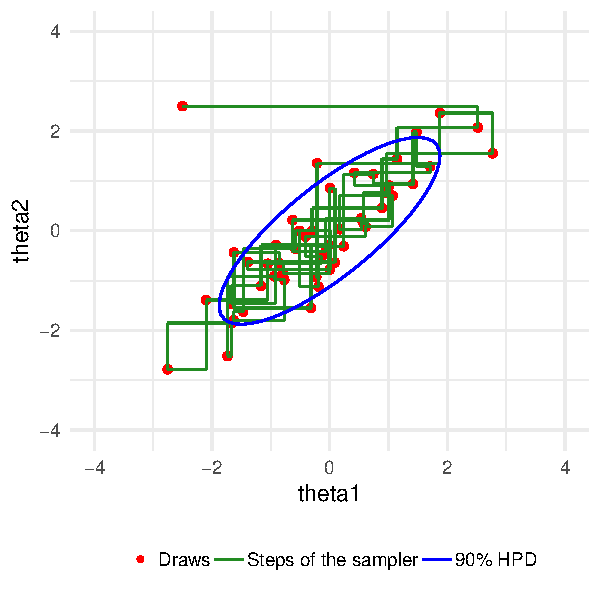
\includegraphics[width=.45\textwidth]{figures/lap4/Gibbs1.pdf}
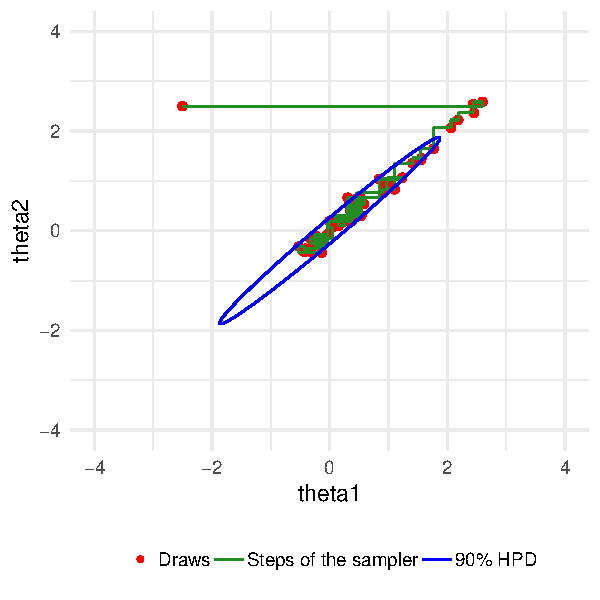
\includegraphics[width=.45\textwidth]{figures/lap4/Gibbs2.pdf}
\end{frame}

\begin{frame}{Gibbs in a 2D Gaussian example}
\centering
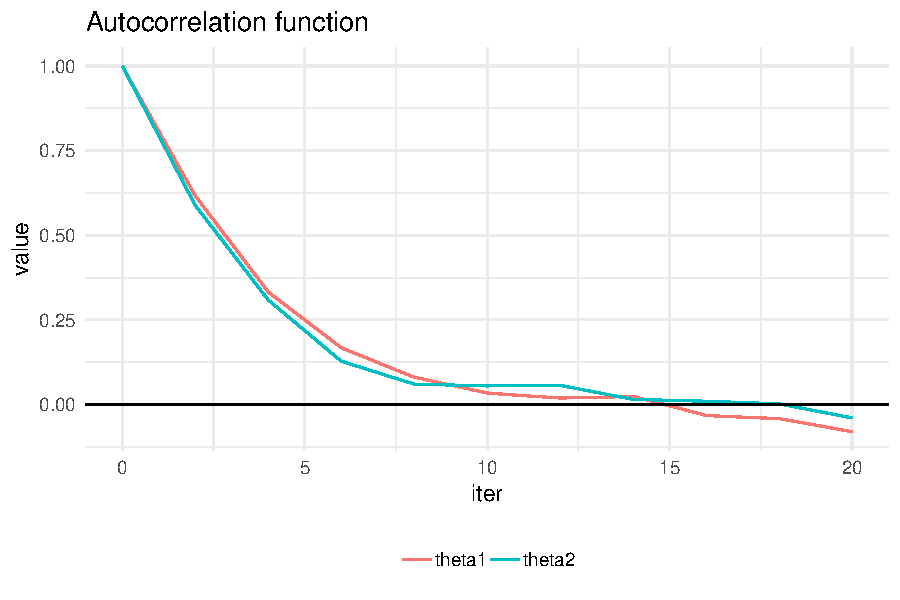
\includegraphics[width=.45\textwidth]{figures/lap4/Gibbs1acf.pdf}
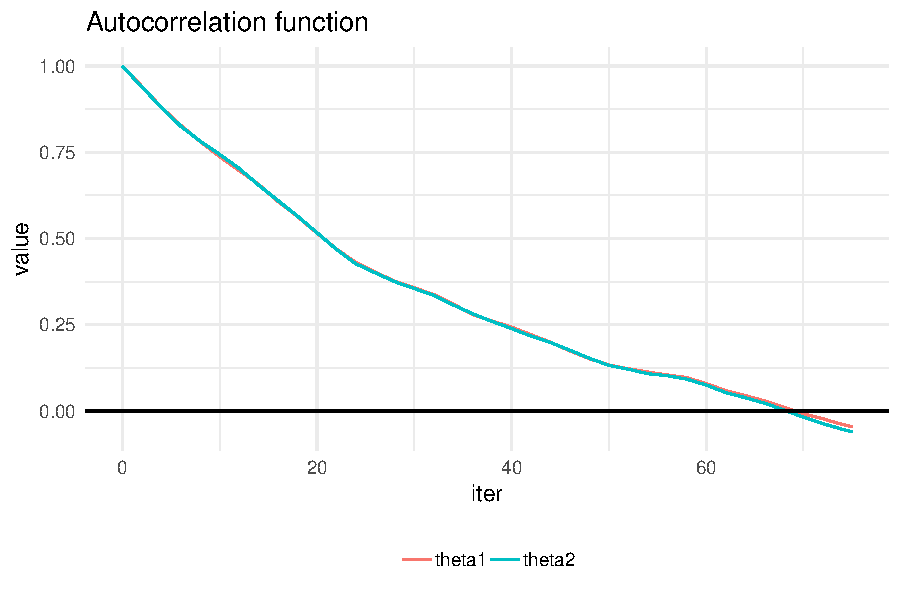
\includegraphics[width=.45\textwidth]{figures/lap4/Gibbs2acf.pdf}
\end{frame}


\section{Criticism: Posterior predictive checks}
\label{sec:ppcs}


\begin{frame}{Lap 4: Bayesian Mixture Models and (Collapsed) Gibbs Sampling}
\begin{itemize}
    \item \hyperref[sec:mixtures]{Model: Bayesian mixture models}
    \item \hyperref[sec:gibbs]{Algorithm: Gibbs sampling}
    \item \hyperref[sec:ppcs]{\textbf{Criticism: Posterior predictive checks}}
    \item \hyperref[sec:collapsed_gibbs]{Algorithm II: Collapsed Gibbs sampling}
\end{itemize}

\vspace{3em}

\begin{center}
    {\Large \textcolor{red}{Slides for this section are adapted from Aki Vehtari's lecture notes.}}
    {\footnotesize \url{https://github.com/avehtari/BDA_course_Aalto/blob/master/slides/}}
\end{center}
\end{frame}


\begin{frame}{Chapter 6 of BDA3: Model checking}
  \begin{itemize}
  \item 6.1 The place of model checking in applied Bayesian statistics
  \item 6.2 Do the inferences from the model make sense?
  \item 6.3 Posterior predictive checking
  \item 6.4 Graphical posterior predictive checks (can be skipped)
  \item 6.5 Model checking for the educational testing example
  \end{itemize}
  
\end{frame}

% \begin{frame}
  
%   {Model checking}

%   \begin{itemize}
%   \item demo6\_1: Posterior predictive checking - light speed
%   \item demo6\_2: Posterior predictive checking - sequential dependence
%   \item demo6\_3: Posterior predictive checking - poor test statistic
%   \item demo6\_4: Posterior predictive checking - marginal predictive p-value
%   \end{itemize}

% \end{frame}

 \begin{frame}{Model checking: Overview}

  \begin{itemize}
  \item<+-> Sensibility with respect to additional information not used in modeling
    \begin{itemize}
    \item e.g., if posterior would claim that hazardous chemical
      decreases probability of death
    \end{itemize}
  \item<+-> External validation
    \begin{itemize}
    \item compare predictions to completely new observations
    \item cf. relativity theory predictions
    \end{itemize}
  \item<+-> Internal validation
    \begin{itemize}
    \item posterior predictive checking
    \item cross-validation predictive checking
    \end{itemize}
  \end{itemize}

\end{frame}

\begin{frame}[fragile]{Posterior predictive checking -- example}

\begin{columns}
  \begin{column}{.5\textwidth}
  \begin{itemize}
  \item<1-> Newcomb's speed of light measurements
    \begin{itemize}
    \item model $y \sim \cN(\mu,\sigma)$ with prior $(\mu,\log\sigma)\propto 1$
    \end{itemize}
    \item<2-> Posterior predictive replicate $y^{\rm rep}$
    \begin{itemize}
    \item<3-> draw $\mu^{(s)},\sigma^{(s)}$ from the posterior $p(\mu,\sigma\mid y)$
    \item<4-> draw $y^{\mathrm{rep}\,(s)}$ from $\cN(\mu^{(s)},\sigma^{(s)})$
    \item<5-> repeat $n$ times to get $y^{\mathrm{rep}}$ with $n$ replicates\\~\\
    \end{itemize}
    \end{itemize}
  \end{column}
  
  \begin{column}{.5\textwidth}
  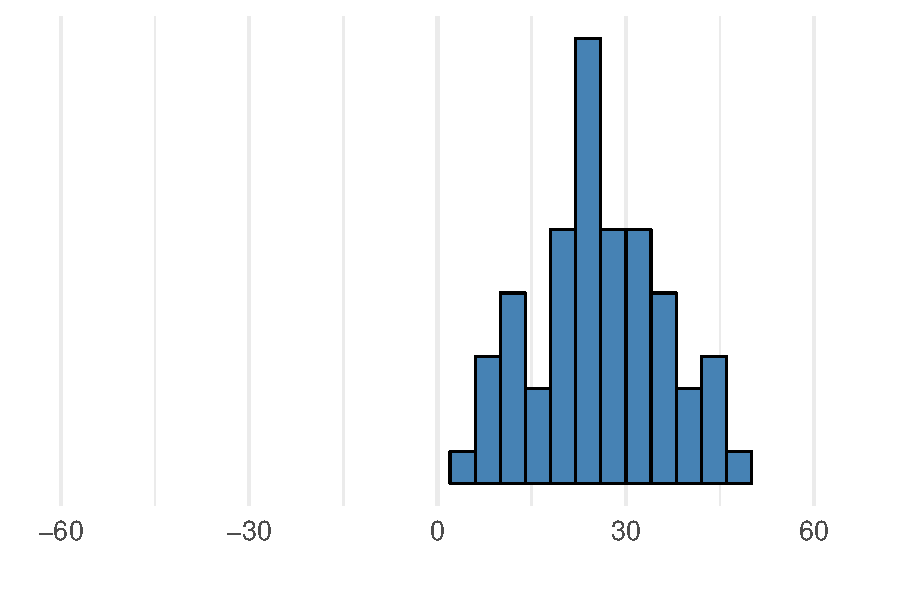
\includegraphics[width=\textwidth]{figures/lap4/light_ppc_1hist.pdf}
  \end{column}
\end{columns}

\end{frame}

\begin{frame}{Replicates vs. future observation}

  \begin{itemize}
  \item Predictive $\tilde{y}$ is the next not yet observed possible
    observation. $y^{\mathrm{rep}}$ refers to replicating the whole
    experiment (potentially with same values of $x$) and obtaining as
    many replicated observations as in the original data.
  \end{itemize}

\end{frame}

\begin{frame}[fragile]{Posterior predictive checking -- example}

  \begin{itemize}
  \item<1-> Generate several replicated datasets $y^{\rm rep}$
  \item<2-> Compare to the original dataset
  \end{itemize}
  \vspace{-1\baselineskip}
  \uncover<3->{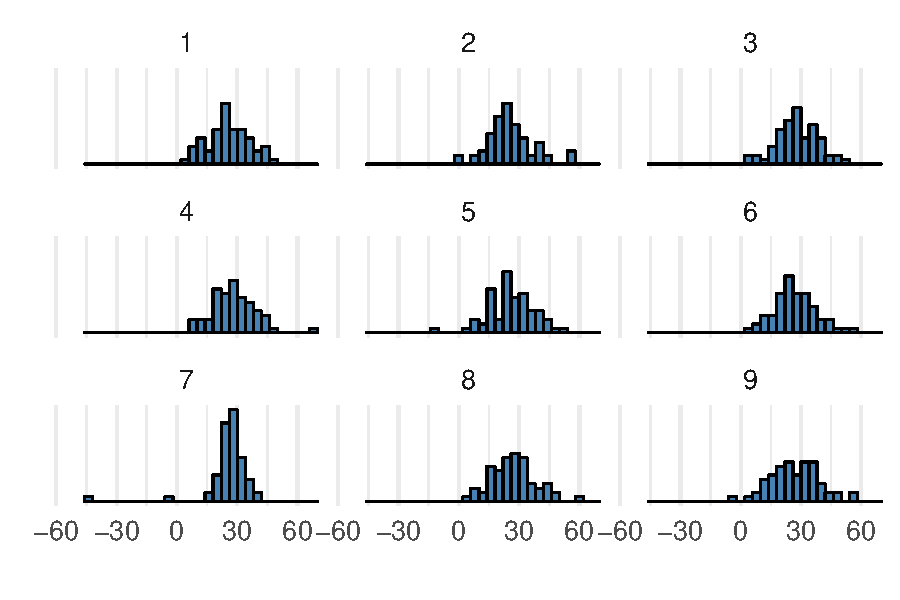
\includegraphics[width=11.5cm]{figures/lap4/light_ppc_10hist.pdf}}

\end{frame}


\begin{frame}{Posterior predictive checking with test statistic}

  \begin{itemize}
  \item Replicated data sets $y^{\mathsf{rep}}$
  \item Test quantity (or discrepancy measure) $T(y,\theta)$
    \begin{itemize}
    \item summary quantity for the observed data $T(y,\theta)$
    \item summary quantity for a replicated data $T(y^{\mathsf{rep}},\theta)$
    \item can be easier to compare summary quantities than data sets
    \end{itemize}
  \end{itemize}

\end{frame}

\begin{frame}[fragile]{Posterior predictive checking -- example}

  \begin{itemize}
  \item<1-> Compute test statistic for data $T(y,\theta)=\min(y)$
  \item<2-> Compute test statistic $\min(y^{\rm rep})$ for many replicated datasets 
  \end{itemize}
  \vspace{-1.5\baselineskip}
  \uncover<3->{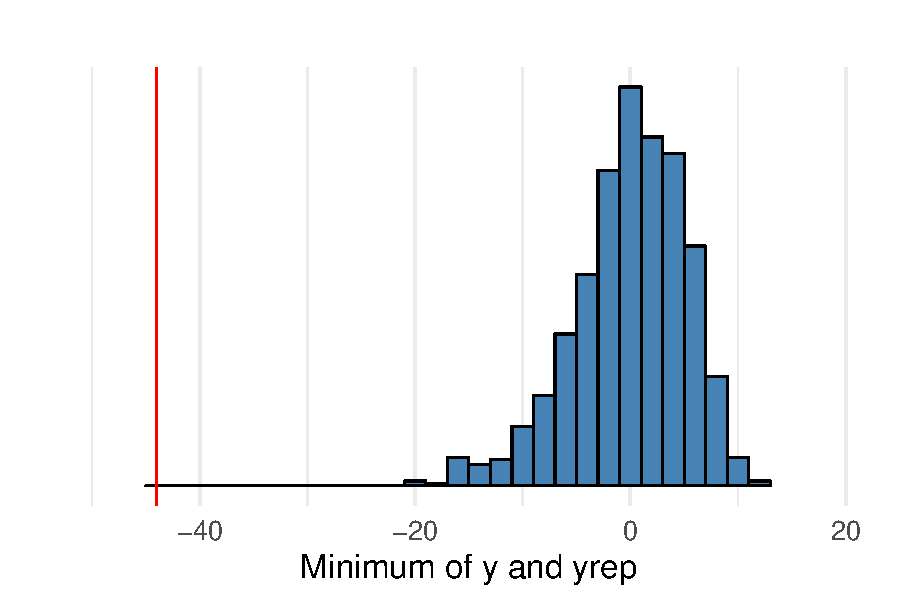
\includegraphics[width=11cm]{figures/lap4/light_ppc_min.pdf}}

\end{frame}

% \begin{frame}[fragile]{Posterior predictive checking -- example}

%   \begin{itemize}
%   \item<1-> Good test statistic is ancillary (or almost)
%     \begin{itemize}
%     \item ancillary if it depends only on observed data and if its
%       distribution is independent of the parameters of the model
%     \end{itemize}
%   \item<2-> Bad test statistic is highly dependent of the parameters
%     \begin{itemize}
%     \item e.g. variance for normal model
%     \end{itemize}
%   \end{itemize}
%   \vspace{-1.5\baselineskip}
%   \uncover<3->{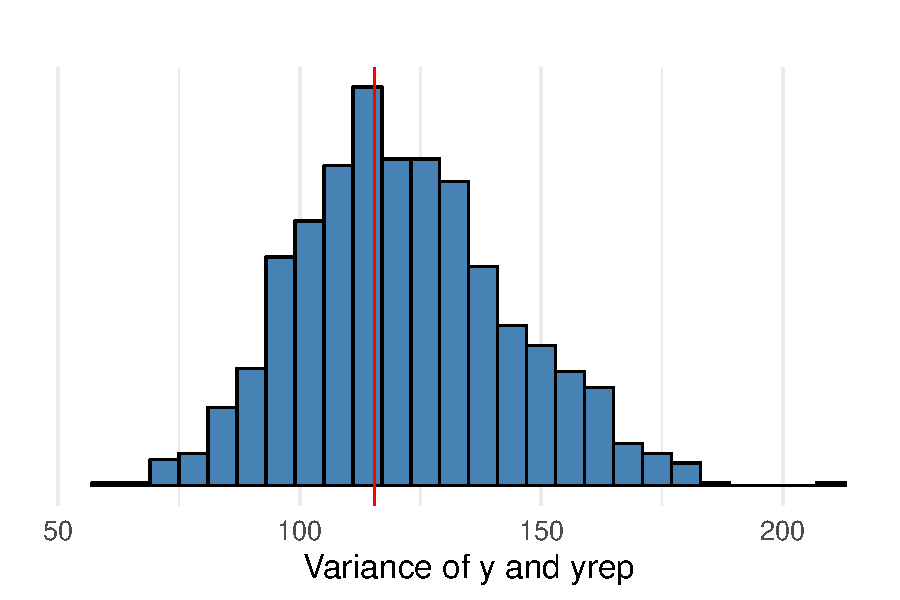
\includegraphics[width=10cm]{figures/lap4/light_ppc_var.pdf}}

% \end{frame}

\begin{frame}[fragile]{Posterior predictive checking}

  \begin{itemize}
    \only<4->{\color{gray}}
  \item<1-> \textit{Posterior predictive $p$-value}
    \begin{eqnarray*}
      p & = & \Pr(T(y^{\mathsf{rep}},\theta)\geq T(y,\theta)\mid y)\\
      & = & \int\int
      \bbI[T(y^{\mathsf{rep}},\theta)\geq T(y,\theta)] \, p(y^{\mathsf{rep}}\mid \theta)p(\theta \mid y)dy^{\mathsf{rep}}d\theta
    \end{eqnarray*}
    where $I$ is an indicator function
    \begin{itemize}
    \item<2-> \only<4->{\color{gray}} having $(y^{\mathsf{rep}\,(s)},\theta^{(s)})$ from the posterior predictive
      distribution, easy to compute
      \begin{equation*}
        T(y^{\mathsf{rep} (s)},\theta^{(s)})\geq T(y,\theta^{(s)}), \quad s=1,\ldots,S
      \end{equation*}
    \end{itemize}
    \vspace{-1.5\baselineskip}
  \item<3-> Posterior predictive $p$-value (ppp-value) estimated whether
    difference between the model and data could arise by chance
  \item<4-> \color{black} Not commonly used, since the distribution of test
    statistic has more information
  \end{itemize}

\end{frame}


% \begin{frame}

%   {Calibration of ppp-values}

%   \begin{itemize}
%   \item In the special case that the parameters $\theta$ are known (or
%     estimated to a very high precision) or in which the test statistic
%     $T(y)$ is ancillary (that is,
%     if it depends only on observed data and if its distribution is
%     independent of the parameters of the model) with a continuous
%     distribution, the posterior predictive $p$-value
%     $\Pr(T(y^{\mathsf{rep}})\!>\!T(y) \mid y)$ has a distribution that is uniform
%     if the model is true.
%   \item Under these conditions, $p$-values less than 0.1 occur 10\% of
%     the time, $p$-values less than 0.05 occur 5\% of the time, and so
%     forth.
%   \end{itemize}

% \end{frame}

% \begin{frame}[fragile]{Marginal and CV predictive checking}

%   \begin{itemize}
%   \item Consider marginal predictive distributions $p(\tilde{y}_i \mid y)$
%     and each observation separately
%     \begin{itemize}
%     \item marginal posterior p-values
%       \begin{align*}
%         p_i = \mbox{Pr}(T(y_i^{\mathsf{rep}}) \leq T(y_i) \mid y)
%       \end{align*}
%       if $T(y_i)=y_i$
%       \begin{align*}
%         p_i = \mbox{Pr}(y_i^{\mathsf{rep}} \leq y_i \mid y)
%       \end{align*}
%     \end{itemize}
%   \item<2-> if $Pr(\tilde{y}_i \mid y)$ well calibrated, distribution of $p_i$
%     would be uniform between 0 and 1
%     \begin{itemize}
%     \item holds better for cross-validation predictive tests
%       (cross-validation Ch 7) 
%     \end{itemize}
%   \end{itemize}

% \end{frame}

% \begin{frame}[fragile]{Marginal predictive checking - Example}

%   \begin{itemize}
%   \item Marginal tail area or Probability integral transform (PIT)
%     \begin{align*}
%       p_i = p(y_i^{\mathsf{rep}} \leq y_i \mid  y)
%     \end{align*}
%   \item if $p(\tilde{y}_i\mid y)$ is well calibrated, distribution of $p_i$'s
%     would be uniform between 0 and 1
%   \end{itemize}
%   \vspace{-1.5\baselineskip}
%   \uncover<2->{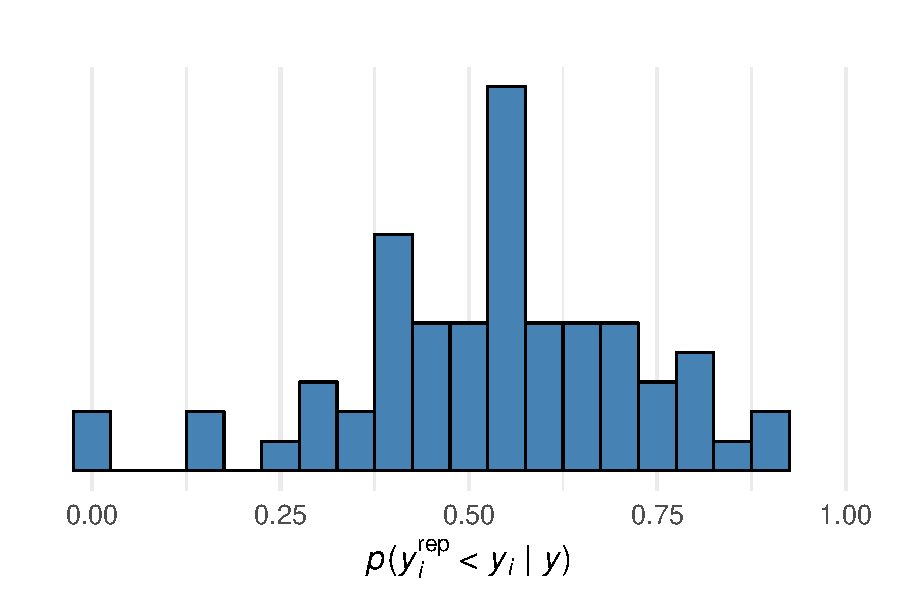
\includegraphics[width=10cm]{figures/lap4/light_ppc_pit.pdf}}

% \end{frame}

\begin{frame}{Sensitivity analysis}

  \begin{itemize}
  \item How much different choices in model structure and priors affect the results
    \begin{itemize}
      \item<2-> test different models and priors
      \item<3-> alternatively combine different models to one model
        \begin{itemize}
        \item e.g. hierarchical model instead of separate and pooled
        \item e.g. $t$ distribution contains Gaussian as a special case
      \end{itemize}
      \item<3-> robust models are good for testing sensitivity to ``outliers''
        \begin{itemize}
        \item e.g. $t$ instead of Gaussian
        \end{itemize}
    \end{itemize}
    \item<4-> Compare sensitivity of essential inference quantities
      \begin{itemize}
      \item extreme quantiles are more sensitive than means and medians
      \item extrapolation is more sensitive than interpolation
      \end{itemize}
    \end{itemize}

\end{frame}


\section{Algorithm II: Collapsed Gibbs Sampling}
\label{sec:collapsed_gibbs}

\begin{frame}{Lap 4: Bayesian Mixture Models and (Collapsed) Gibbs Sampling}
\begin{itemize}
    \item \hyperref[sec:mixtures]{Model: Bayesian mixture models}
    \item \hyperref[sec:gibbs]{Algorithm: Gibbs sampling}
    \item \hyperref[sec:ppcs]{Criticism: Posterior predictive checks}
    \item \hyperref[sec:collapsed_gibbs]{\textbf{Algorithm II: Collapsed Gibbs sampling}}
\end{itemize}
\end{frame}

% Also, augmentation to render models conjugate
\begin{frame}{``Collapsing'' out variables}
In some models, we can marginalize (aka \textit{collapse} or \textit{integrate out}) some variables to work on a lower dimensional distribution. 

Typically, this is possible in models constructed with conjugate exponential family distributions.
    
\end{frame}

\begin{frame}{Collapsed Gibbs for Bayesian mixtures}
    Let's marginalize the parameters $\{\mbeta_k\}_{k=1}^K$ in the exponential family mixture model,
    \begin{align}
        p(\mbpi, &\{(z_n, \mbx_n)\}_{n=1}^N \mid \mbphi, \nu, \mbalpha) 
        =
        \distDirichlet(\mbpi \mid \mbalpha) \prod_{k=1}^K \left[ \int p(\mbeta_k \mid \mbphi, \nu) \, \prod_{n=1}^N \left[ \pi_k \, p(\mbx_n \mid \mbeta_k) \right]^{\bbI[z_n = k]} \dif \mbeta_k \right] \\
        &\propto
        \distDirichlet(\mbpi \mid \mbalpha) \prod_{k=1}^K \left[ \pi_k^{N_k} \int \frac{1}{Z_{\mbeta}(\mbphi, \nu)} \exp \left\{\Big\langle \mbphi + \sum_{n: z_n=k} t(\mbx_n), \mbeta_k \Big\rangle - (\nu + N_k) A(\mbeta_k) \right\}  \dif \mbeta_k \right] \\
        &=
        \distDirichlet(\mbpi \mid \mbalpha) \prod_{k=1}^K \left[ \pi_k^{N_k} \frac{Z_{\mbeta}(\mbphi + \sum_{n: z_n=k} t(\mbx_n), \nu + N_k)}{Z_{\mbeta}(\mbphi, \nu)} \right]
    \end{align}
    where $Z_{\mbeta}(\mbphi, \nu)$ is the normalizing function of the conjugate prior $p(\mbeta \mid \mbphi, \nu)$.
    
    \textbf{Question: } can we still parallelize the Gibbs updates of $\{z_n\}_{n=1}^N$?
\end{frame}

\begin{frame}{Collapsed Gibbs for Bayesian mixtures II}
    While we're at it, let's marginalize the mixture proportions $\mbpi$, too. The Dirichlet density is,
    \begin{align}
        \distDirichlet(\mbpi \mid \mbalpha) 
        &= \frac{1}{Z_{\mbpi}(\mbalpha)} \prod_{k=1}^K \pi_k^{\alpha_k - 1} 
        \quad \text{where} \quad
        Z_{\mbpi}(\mbalpha) = \frac{\prod_{k=1}^K \Gamma(\alpha_k)}{\Gamma(\sum_{k=1}^K \alpha_k)}
    \end{align}
    Plugging this in and integrating over $\mbpi$ yields,
    \begin{align}
        p(\{(z_n, \mbx_n)\}_{n=1}^N \mid \mbphi, \nu, \mbalpha) 
        &=
        \left[ \int \distDirichlet(\mbpi \mid \mbalpha) \prod_{k=1}^K \pi_k^{N_k} \dif \mbpi \right] 
        \left[ \prod_{k=1}^K \frac{Z_{\mbeta}(\mbphi + \sum_{n: z_n=k} t(\mbx_n), \nu + N_k)}{Z_{\mbeta}(\mbphi, \nu)} \right] \\
        &=
        \left[ \frac{Z_{\mbpi}([\alpha_1 + N_1, \ldots, \alpha_K + N_K])}{Z_{\mbpi}(\mbalpha)} \right] 
        \left[ \prod_{k=1}^K \frac{Z_{\mbeta}(\mbphi + \sum_{n: z_n=k} t(\mbx_n), \nu + N_k)}{Z_{\mbeta}(\mbphi, \nu)} \right] 
    \end{align}
\end{frame}

\begin{frame}{Collapsed Gibbs for Bayesian Mixtures III}
We'll simplify the notation by writing,
\begin{align}
    p(\{(z_n, \mbx_n)\}_{n=1}^N \mid \mbphi, \nu, \mbalpha) 
    &=
    \frac{Z_{\mbpi}(\mbalpha')}{Z_{\mbpi}(\mbalpha)}
    \prod_{k=1}^K \frac{Z_{\mbeta}(\mbphi_k', \nu_k')}{Z_{\mbeta}(\mbphi, \nu)}
\end{align}
where 
\begin{align}
    \mbalpha' &= [\alpha_1 + N_1, \ldots, \alpha_K + N_K] \\
    \mbphi_k' &= \mbphi + \sum_{n: z_n=k} t(\mbx_n)\\
    \nu_k' &= \nu + N_k.
\end{align}
This is a \textbf{general pattern}: in exponential families, marginal likelihoods are given by ratios of posterior and prior normalizing functions.
\end{frame}

\begin{frame}{Collapsed Gibbs for Bayesian Mixtures IV}
Now consider the conditional distribution of $z_n$, holding all the other assignments fixed,
\begin{align}
    p(z_n=k \mid \mbx_n, \{(z_n, \mbx_n)\}_{n' \neq n}, \mbphi, \nu, \mbalpha) 
    &\propto
    Z_{\mbpi}(\mbalpha') \prod_{k=1}^K Z_{\mbeta}(\mbphi_k', \nu_k')
\end{align}
where $\mbalpha'$, $\mbphi_k'$, and $\nu_k'$ are computed with $z_n=k$. To simplify, divide by a constant w.r.t. $z_n$,
\begin{align}
    p(z_n=k \mid \mbx_n, \{(z_n, \mbx_n)\}_{n' \neq n}, \mbphi, \nu, \mbalpha) 
    &\propto
    \frac{Z_{\mbpi}(\mbalpha')}{Z_{\mbpi}(\mbalpha'^{(\neg n)})} \prod_{k=1}^K \frac{Z_{\mbeta}(\mbphi_k', \nu_k')}{Z_{\mbeta}(\mbphi_k'^{(\neg n)}, \nu_k'^{(\neg n)})}
\end{align}
where
\begin{align}
    \mbalpha'^{(\neg n)} &= [\alpha_1 + N_1^{(\neg n)}, \ldots, \alpha_K + N_K^{(\neg n)}] &
    \mbphi_k'^{(\neg n)} &= \mbphi + \sum_{n' \neq n} t(\mbx_{n'}) \bbI[z_{n'}=k] \\
    \nu_k'^{(\neg n)} &= \nu + N_k^{(\neg n)} &
    N_k^{(\neg n)} &= \sum_{n' \neq n} \bbI[z_{n'} = k]
\end{align}

\end{frame}

\begin{frame}{Collapsed Gibbs for Bayesian Mixtures V}
Then many terms cancel. In the first ratio,
\begin{align}
    \frac{Z_{\mbpi}(\mbalpha')}{Z_{\mbpi}(\mbalpha'^{(\neg n)})} &= \frac{\prod_{k=1}^K \Gamma(\alpha_k') \, \Gamma(\sum_{k=1}^K \alpha_{k}'^{(\neg n)})}{\prod_{k=1}^K \Gamma(\alpha_k'^{(\neg n)}) \, \Gamma(\sum_{k=1}^K \alpha_{k}')} 
    \propto \alpha_k'^{(\neg n)} = \alpha + N_k^{(\neg n)}
\end{align}
In words, the first ratio is proportion to the size of cluster $k$ before adding the $n$-th data point.

Consider the second ratio. All but the $k$-th term in the product cancel to leave:
\begin{align}
    \prod_{k=1}^K \frac{Z_{\mbeta}(\mbphi_k', \nu_k')}{Z_{\mbeta}(\mbphi_k'^{(\neg n)}, \nu_k'^{(\neg n)})} 
    = \frac{Z_{\mbeta}(\mbphi_k', \nu_k')}{Z_{\mbeta}(\mbphi_k'^{(\neg n)}, \nu_k'^{(\neg n)})}
    &\propto p(\mbx_n \mid \{\mbx_{n'}: z_{n'} = k\}, \mbphi, \nu).
\end{align}
In words, the second ratio is proportional to the \textit{posterior predictive density}.

Altogether, the conditional distribution of $z_n$ is,
\begin{align}
    p(z_n=k \mid \mbx_n, \{(z_n, \mbx_n)\}_{n' \neq n}, \mbphi, \nu, \mbalpha) 
    &\propto (\alpha_k + N_k^{(\neg n)}) \, p(\mbx_n \mid \{\mbx_{n'}: z_{n'} = k\}, \mbphi, \nu),
\end{align}
a function of the size of the cluster and the likelihood of $\mbx_n$ given other points in that cluster.

\end{frame}

\begin{frame}{The infinite limit: Dirichlet process mixture models}
Now consider a special case where $\mbalpha = \tfrac{\alpha}{K} \mbone_K$ and, loosely speaking, take $K \to \infty$. In this limit, we obtain a \textbf{Dirichlet process mixture model}. 

There's lots of theory about these Bayesian nonparametric models that we won't touch on today~\citep[see][]{orbanz2012lecture}. Instead, just note how the collapsed Gibbs sampling algorithm changes.

The probability of assigning the $n$-th data point to a non-empty cluster is still,
\begin{align}
    p(z_n=k \mid \mbx_n, \{(z_n, \mbx_n)\}_{n' \neq n}, \mbphi, \nu, \mbalpha) 
    &\propto (\frac{\alpha}{K} + N_k^{(\neg n)}) \, p(\mbx_n \mid \{\mbx_{n'}: z_{n'} = k\}, \mbphi, \nu).
\end{align}
But now there are only $K_{\mathsf{used}} = \# \mathrm{unique}(\{z_{n'}\}_{n' \neq n})$ non-empty clusters, and the remaining $K - K_{\mathsf{used}}$ unoccupied clusters each have probability, 
\begin{align}
    p(z_n=k \mid \mbx_n, \{(z_n, \mbx_n)\}_{n' \neq n}, \mbphi, \nu, \mbalpha) 
    &\propto \tfrac{\alpha}{K} \, p(\mbx_n \mid \mbphi, \nu).
\end{align}

\end{frame}

\begin{frame}{The infinite limit: Dirichlet process mixture models II}
Since all the empty clusters are equivalent, we can combine them to get,
\begin{multline}
    p(z_n=k \mid \mbx_n, \{(z_n, \mbx_n)\}_{n' \neq n}, \mbphi, \nu, \mbalpha) 
    \\
    \propto 
    \begin{cases}
    (\frac{\alpha}{K} + N_k^{(\neg n)}) \, p(\mbx_n \mid \{\mbx_{n'}: z_{n'} = k\}, \mbphi, \nu) & \text{if } k \in \{1, \ldots, K_{\mathsf{used}} \} \\
    (K - K_{\mathsf{used}}) \tfrac{\alpha}{K} \, p(\mbx_n \mid \mbphi, \nu) & \text{if } k = K_{\mathsf{used}} + 1,
    \end{cases}
\end{multline}
where we assume that the cluster labels are permuted after each iteration so that only $k=1, \ldots, K_{\mathsf{used}}$ are non-empty. 

As $K \to \infty$, these updates simplify to the classic collapsed Gibbs updates for DPMMs,
\begin{multline}
    p(z_n=k \mid \mbx_n, \{(z_n, \mbx_n)\}_{n' \neq n}, \mbphi, \nu, \mbalpha) 
    \\
    \propto 
    \begin{cases}
    N_k^{(\neg n)} \, p(\mbx_n \mid \{\mbx_{n'}: z_{n'} = k\}, \mbphi, \nu) & \text{if } k \in \{1, \ldots, K_{\mathsf{used}} \} \\
    \alpha \, p(\mbx_n \mid \mbphi, \nu) & \text{if } k = K_{\mathsf{used}} + 1.
    \end{cases}
\end{multline}
\end{frame}

\begin{frame}{The infinite limit: Dirichlet process mixture models III}
As the Gibbs sampler runs, it has some probability of deleting a cluster (by removing its last data point) and some probability (determined by $\alpha$) of creating a new cluster with one data point. In this sense, the model is \textbf{nonparametric}: it doesn't require you to specify $K$ in advance. 

These probabilities are \textit{size-biased}, you're more likely to add a data point to a large cluster.

There are many other ways to arrive at the DPMM:
\begin{enumerate}
    \item via an stochastic process on partitions called the \textbf{Chinese restaurant process (CRP)}
    \item as a \textbf{random measure} on $\mbeta$ with a countably infinite number of weighted atoms, only a finite number of which are used.
    \item via a \textbf{stick-breaking construction} to get the weights of the random measure.
\end{enumerate}
\citet{orbanz2012lecture} offers an accessible, book-length treatment of these important models.

\end{frame}

% Random measure perspective

\begin{frame}[t,allowframebreaks]
        \frametitle{References}
        \bibliographystyle{unsrtnat}
        \bibliography{refs.bib}
\end{frame}

\end{document}